\subsection{Why is Software Management important?}
\label{sec:software_management}
In Software Development, it is said that the speed of work is often dictated by
the quality of the tools used to perform that work. Knowing this,
\textit{Magpie} makes use of a number of tools to ensure that the development
process is as efficient as possible.

This chapter will discuss the tools we used to create \textit{Magpie} and how
they were used to manage the project. We will also discuss the importance of the
tools used and how they helped aid development and maintain a solid pace.

\subsection{What is DevOps?}
\label{sec:devops}

\begin{quote}
    ``DevOps is about fast, flexible development and provisioning business
    processes. It efficiently integrates development, delivery, and operations,
    thus facilitating a lean, fluid connection of these traditionally separated
    silos''
    \cite{DevOps}
\end{quote}

\textbf{DevOps} is a set of principles and practices that combines software
development \textbf{(Dev)} and IT operations \textbf{(Ops)}. The primary means
of reducing friction between development and operations is through automation,
and the use of tools to multiply progress, and reduce effort. This can be
broadly sorted into two categories:

\begin{itemize}
    \item{\textbf{Continuous Integration (CI)}: This is the practice of
        automatically building and testing code every time a developer commits
        changes to version control. This ensures that the code is always in a
        working state. \cite{DevOps}.}
        \vspace{1em}
    \item{\textbf{Continuous Deployment (CD)}: This is the practice of
        automatically deploying code to production servers every time a change
        is made. This ensures that the application is always up–to–date and that
        new features can be released quickly. \cite{DevOps}.}
\end{itemize}

The next sections will detail the tools used to implement
\textbf{Continuous Integration} and \textbf{Continuous Deployment.}

\subsection{Continuous Integration}
\label{sec:continuous_integration}
In \textit{Magpie}, the CI workflow is focused around \textbf{GitHub} and it's
suite of tools. We decided on using this approach, because it enables a powerful
flow:

\begin{figure}[htbp]
    \centering{}
    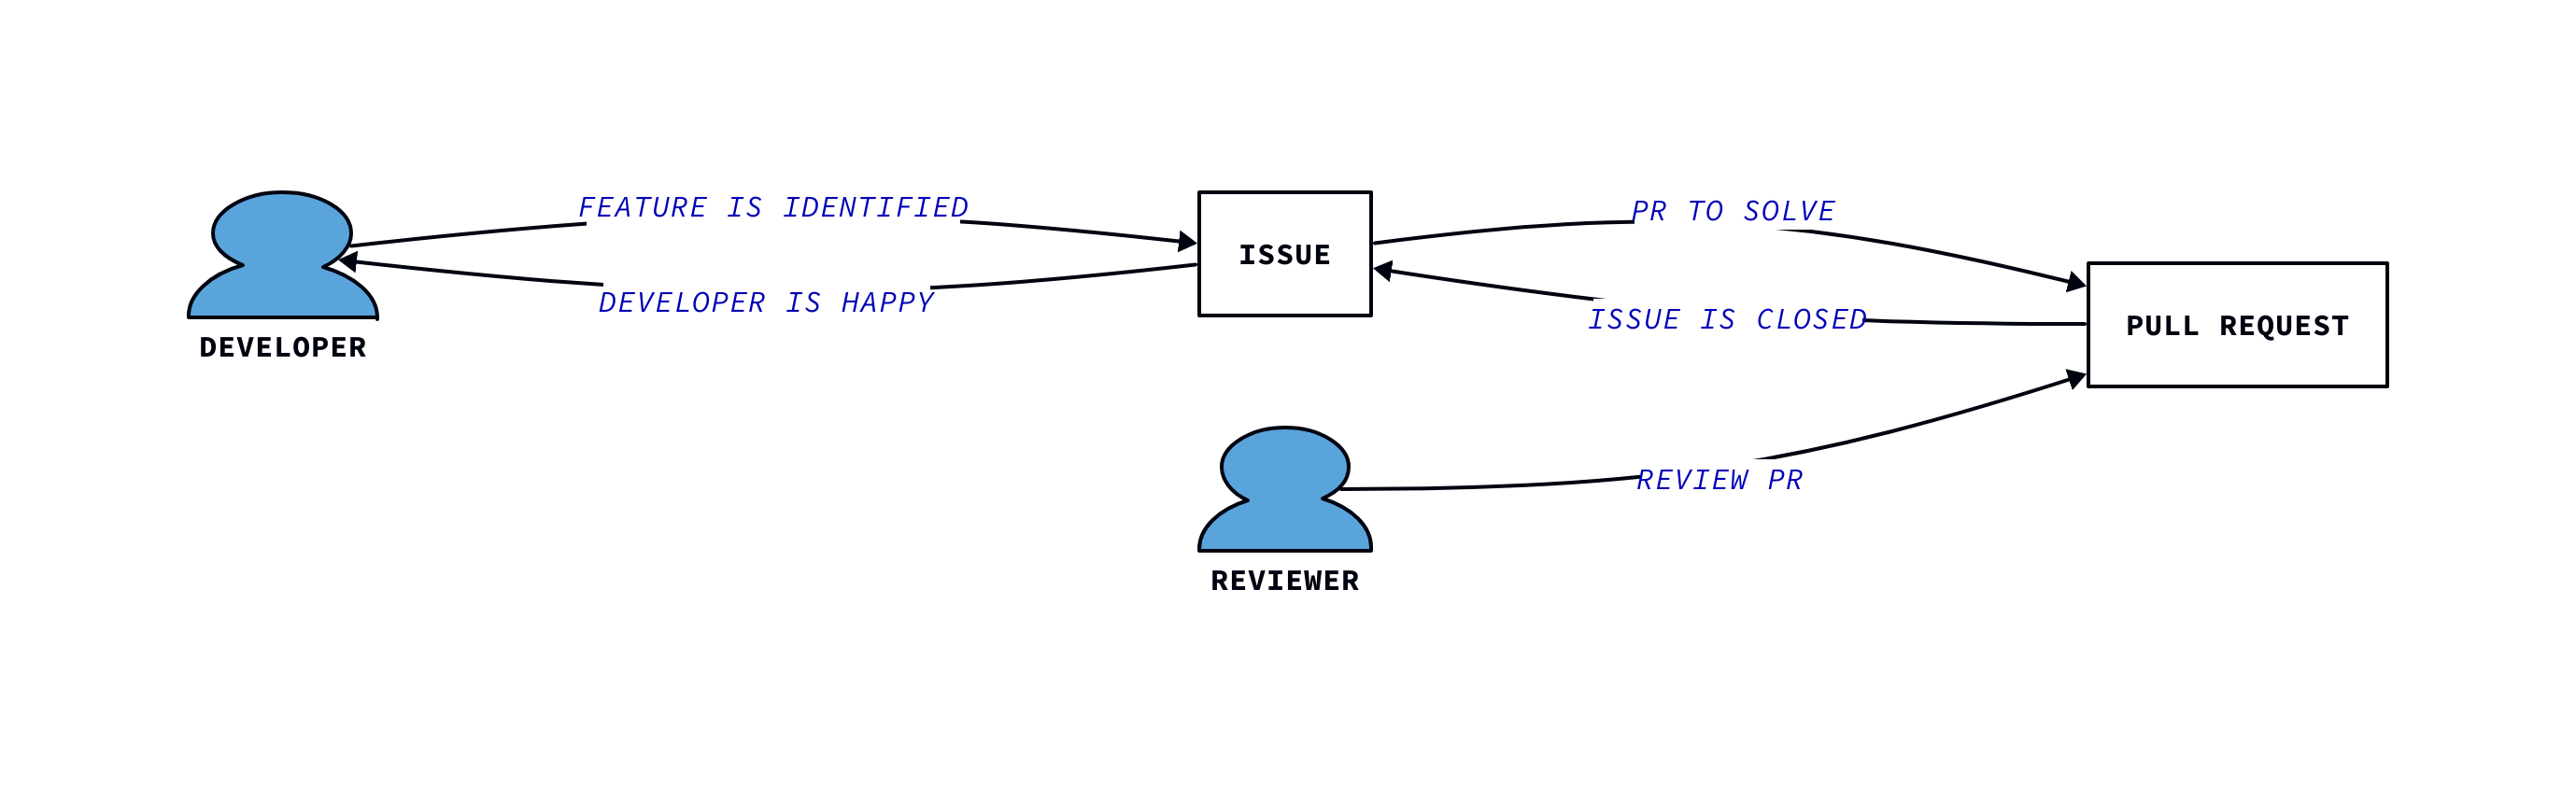
\includegraphics[width=\textwidth]{../d2-diagrams/issues-prs/diagram.png}
    \caption{The flow of work in \textit{Magpie}}
\end{figure}

\subsubsection{Issues}
\label{sec:github_issues}
\textbf{GitHub Issues} are used to track tasks, enhancements, and bugs to be
worked on. In our experience, they are a effective way to keep track of what
needs to be done, and what has been done. \textbf{GitHub Issues} can be assigned
to team members, and can be linked to \textbf{Pull Requests}.

Issues represent the primary unit of work in projects using \textbf{GitHub}'s
flow. In the below example, a checklist is presented- with each item indicating
a task that needs to be completed. An issue's checkboxes, can also be assigned
to \textbf{Pull Requests}.

On the right, the issue displays the \textbf{Assignees}, \textbf{Labels}, and
\textbf{Projects} associated with the issue. This allows for easy filtering and
sorting of issues, and helps to keep the project organized.

Under the description, the issue keeps track of edits, comments, and other
interactions. This allows for communication to stay in context with the issue
being discussed, and requirements- or additional information- to be added as
needed.

\begin{figure}[htbp]
    \centering{}
    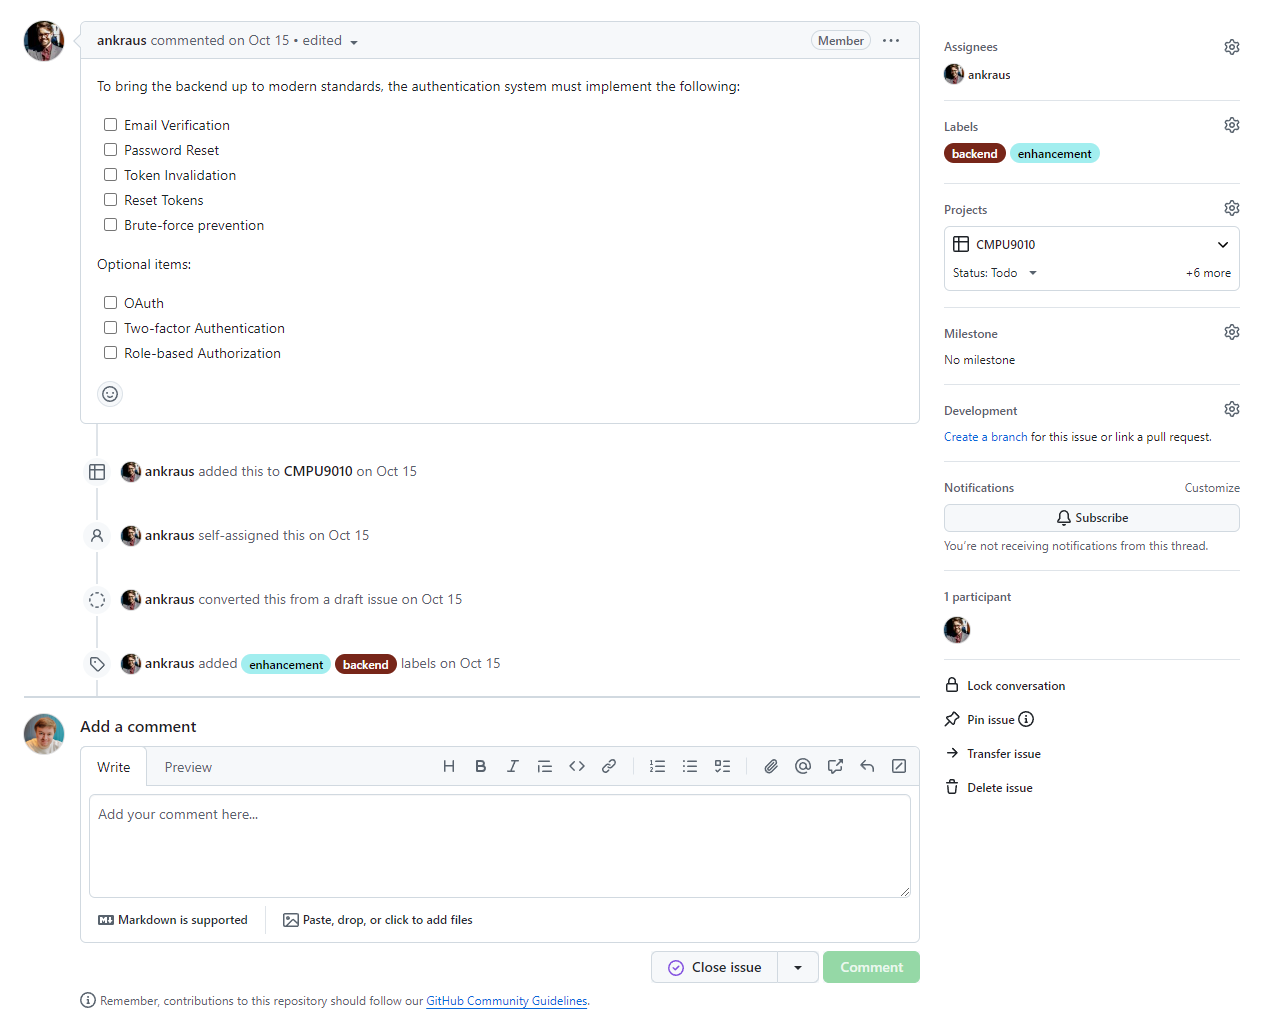
\includegraphics[width=\textwidth]{images/github_issue.png}
    \caption{An example of a GitHub Issue}
\end{figure}

\newpage{}

In general, issues are a great way to keep track of what needs to be done,
however, in our experience, they can be tedious to write manually. To help with
this, templates can be used.

To use a template, create a directory called \textbf{.github} in the root of the
project, then create another directory called \textbf{ISSUE\_TEMPLATE}, note
that the capitalization is important. Inside this directory, any markdown file
created in the prescribed format can be used as a template for issues, you can
have as many templates as you like.

In \textit{Magpie}, we used a template for \textbf{Bug Reports},
\textbf{Documentation Requests}, and \textbf{Feature Requests}. This reduced the
friction of creating issues by minimising the amount of effort related to
drafting an issue (using the template) and creating clear delineations between
different categories of issues.

\begin{listing}[htbp]
    \centering{}
    \begin{minted}{html}
        ---
        name: Bug Report
        about: Create a report to help us improve
        title: ''
        labels: bug
        assignees: ''
        ---

        **Describe the bug**
        A clear and concise description of what the bug is.

        **To Reproduce**
        Steps to reproduce the behavior:

        1. Go to '...'
        2. Click on '....'
        3. Scroll down to '....'
        4. See error

        **Expected behaviour**
        A clear and concise description of what you expected to happen.

        **Screenshots**
        If applicable, add screenshots to help explain your problem.

        **Additional context**
        Add any other context about the problem here.
    \end{minted}
    \caption{An example of an issue template used in \textit{Magpie}}
\end{listing}

\newpage{}

\subsubsection{Pull Requests}
\textbf{Pull Requests} are used to merge code from one branch to another. In our
experience, they are a great way to review code, and ensure that it is up to
standard. They can be linked to \textbf{Issues}, and like issues, can be
assigned to team members.

In the below example, the interface is largely similar to that of an issue,
however there are a few key differences. Note that under projects, you can set a
task that will be present in the Kanban board that will be discussed in the next
section.

If this PR solves a milestone, or contributes to an issue containing a
milestone, it will be displayed here. \textit{Magpie} did not use milestones
with the exception of the interim report, however we feel it can be valuable in
projects with more clearly defined goals, such as major releases.

Note, that the pull requests we used also included automated CI jobs. These will
be discussed in a later section.

\begin{figure}[htbp]
    \centering{}
    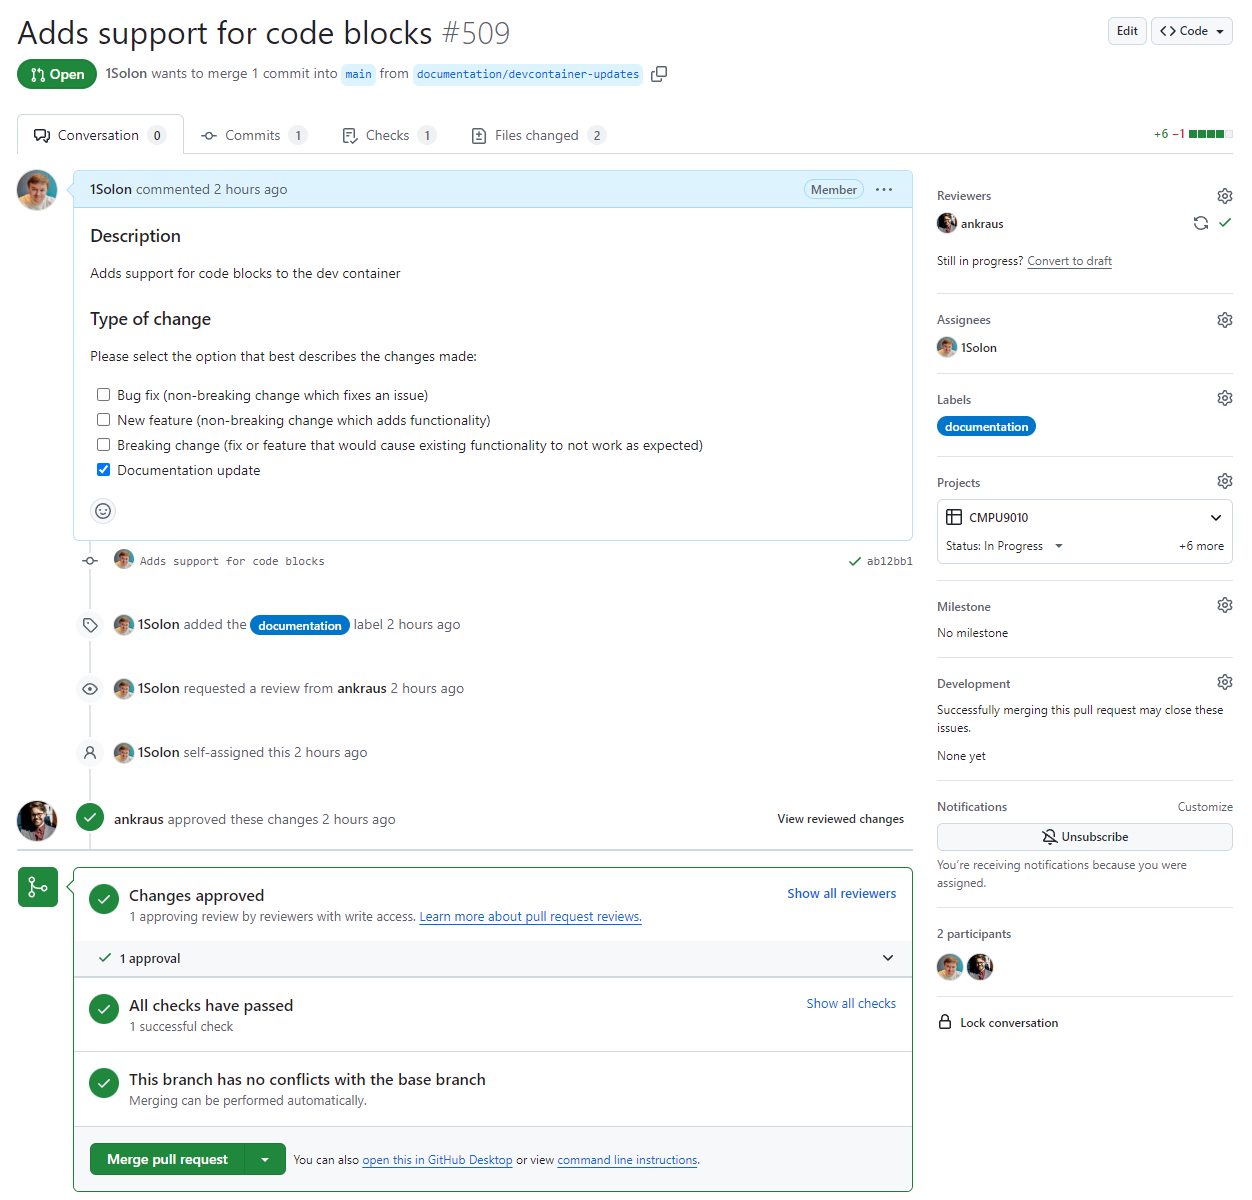
\includegraphics[width=\textwidth]{images/github_pr.png}
    \caption{An example of a GitHub Pull Request}
\end{figure}

\newpage{}

Like \textbf{Issues}, \textit{Magpie} leverages \textbf{Pull Request Templates}
to reduce friction. Templates reduce friction by minimising the amount of
writing necessary when drafting a PR.

During the project, we at times ignored issue templates because because the
benefits of writing fully-detailed issues, did not always return greater
utility. However, we never ignored pull request templates.

PRs need a high level description of the changes made, and having a consistent
format for this description was important to ease the burden on code reviewers,
particularly working in a team environment.

\begin{listing}[htbp]
    \centering{}
    \begin{minted}{html}
        ### Description

        Replace this with a summary of the change. Please also include relevant
        motivation and context.

        Fixes # (issue)

        ### Type of change

        Please select the option that best describes the changes made:

        - [ ] Bug fix (non-breaking change which fixes an issue)
        - [ ] New feature (non-breaking change which adds functionality)
        - [ ] Breaking change (fix or feature that would break existing functionality)
        - [ ] Documentation update

        ### Changes

        Replace this with a list of changes made in the pull request.
    \end{minted}
    \caption{An example of a pull request template used in \textit{Magpie}}
\end{listing}

\newpage{}

\subsubsection{Projects}
\textbf{GitHub Projects} are used to track the progress of work in a project. In
our experience, they are a great way to keep track of what needs to be done, and
what has been done.

\textbf{GitHub Projects} can be used to create a \textbf{Kanban Board}. In our
experience, this is a great way to visualise the progress of work in a project.
In the below example, the board is divided into columns, each representing a
different stage of work.

\begin{figure}[htbp]
    \centering{}
    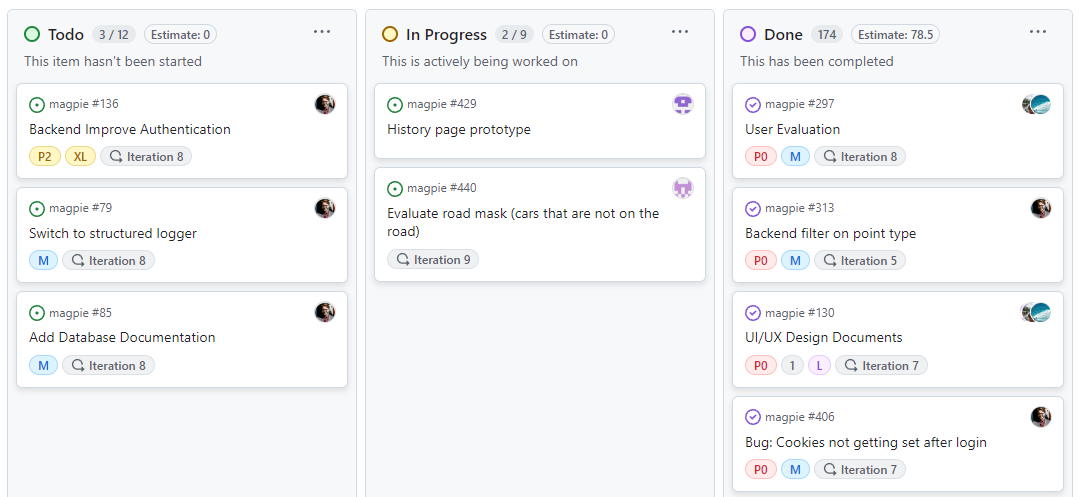
\includegraphics[width=\textwidth]{images/github_kanban.png}
    \caption{An example of a GitHub Kanban Board}
\end{figure}

In \textit{Magpie}, we predominantly used the \textbf{Kanban Board} to provide a
high-level overview of tasks within the project. In general, this allowed all
team members to see what was being worked on, and what needed to be done.

As a card is just a representation of an issue, clicking on it will take you to
the issue page. This closes the loop on the flow identified in the beginning of
this section.

\textbf{GitHub Projects} includes a \textbf{Roadmap} tab. Unlike the
\textbf{Kanban Board} tab, which gives an overview of task status, the
\textbf{Roadmap} gives a temporal view of the timing associated with those
tasks.

\begin{figure}[h]
    \centering{}
    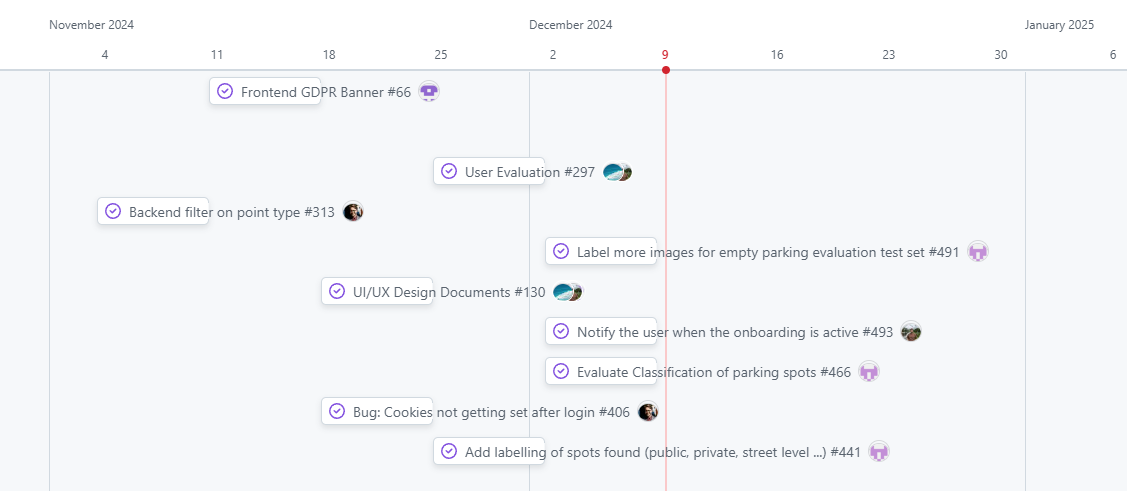
\includegraphics[width=\textwidth]{images/github_roadmap.png}
    \caption{An example of a GitHub Roadmap}
\end{figure}

\newpage{}

\subsection{Actions}
\textbf{GitHub Actions} are used to automate tasks in a project. In
\textbf{Magpie}, we used \textbf{GitHub Actions} to automate tests, housekeeping
and building tasks. Housekeeping and tests fall comfortably within CI, however
building is more closely aligned to CD- as such, it will be discussed in a later
section.

\subsubsection{Houskeeping}
\textbf{Magpie} uses a branch naming scheme:
\begin{itemize}
    \item \textbf{main}: The main branch of the project. This is the branch that
        is deployed to production.
    \item \textbf{backend/}: A branch containing backend features.
    \item \textbf{frontend/}: A branch containing frontend features.
    \item \textbf{documentation/}: A branch containing documentation.
    \item \textbf{python/}: A branch containing Machine Learning features.
    \item \textbf{update/}: A branch containing updates to the project.
    \item \textbf{misc/}: A branch containing anything not in the above categories.
\end{itemize}
This was initially done to trigger specific actions based on the name of the
branch. However, it became a neat means of seeing what branch was dealing with
what task, in our experience, in projects like this with upwards of 8+ branches
at a time, being able to, at-a-glance, determine what the branch was dealing
with was very useful.

We decided against using branch rules to trigger actions because, by default,
they do not function as expected. For example:

\begin{listing}[htbp]
    \centering{}
    \begin{minted}{yaml}
        on:
            push:
                branches:
                - 'feature/*'
    \end{minted}
    \caption{An example of a GitHub Actions workflow that will not work}
\end{listing}

From the above, you may expect that the workflow will trigger on any branches
starting with \textbf{feature/}. However, this will only trigger on any branches
being \textit{merged into} \textbf{feature/}. This is not the desired behaviour,
and as such, we decided against using this particular method.

To solve this problem, we instead triggered actions based on what \textit{directory} was
being changed. This was done by using the \textbf{paths} key in the workflow.

\begin{listing}[htbp]
    \centering{}
    \begin{minted}{yaml}
        on:
            push:
                paths:
                - 'Backend/**'
    \end{minted}
    \caption{An example of a GitHub Actions workflow that will work}
\end{listing}

\newpage{}

In \textit{Magpie}, to maintain our branch naming scheme, it was important to
have automation in place to ensure that branches were named correctly. This was
done using a \textbf{GitHub Action} that would check the branch name, and if it
did not match the scheme, would fail the action.

Note that, in a \textbf{Pull Request}, certain actions will come up as checks. 
Checks will prevent a PR from being merged if they fail.

\begin{listing}[htbp]
    \begin{minted}{yaml}
        name: Branch Checks

        on:
        pull_request:

        jobs:
        validate-name:
            runs-on: ubuntu-latest

            steps:
            - name: Check out repository
                uses: actions/checkout@v4

            - name: Get branch name
                id: get_branch_name
                run: echo "branch=${GITHUB_HEAD_REF}" >> $GITHUB_OUTPUT

            - name: Validate branch name
                run: |
                BRANCH_NAME="${{ steps.get_branch_name.outputs.branch }}"
                if [[ ! "$BRANCH_NAME" =~ ^(
                    backend/ frontend/|
                    documentation/ python/|
                    distribution/ misc/|
                    update/
                    ).* ]]; then
                    echo "Branch name '$BRANCH_NAME' is not valid."
                    echo "Rename the branch to match one of the following patterns:"
                    echo "'backend/', 'frontend/',"
                    echo "'documentation/', 'distribution/',"
                    echo "'update/', 'python/',"
                    echo "or 'misc/'."
                    exit 1
                fi
            shell: bash
    \end{minted}
    \caption{A github action that checks the branch name (this was edited for brevity)}
\end{listing}

The above action runs on every pull request, and checks the branch name. If the
branch name does not match the pattern, the action will fail, and the PR will
not be able to be merged.

\subsubsection{Checks}

\textbf{GitHub Actions} can be used to run checks on code. In \textit{Magpie},
we used checks to run automated testing in the fronted and backend. The frontend
and backend checks are discussed in those sections.

\subsection{Continuous Deployment}

\subsubsection{Kubernetes}
Kubernetes, often abbreviated as \textit{K8s}, is an open-source container
orchestration platform designed to automate the deployment, scaling, and
management of containerized applications.

\begin{itemize}
    \item \textbf{Container Orchestration:} Kubernetes manages the lifecycle of
    containers, ensuring that applications are running as intended and
    automatically handling failures or restarts.
    \item \textbf{Scalability:} It supports horizontal scaling of applications
    through commands, resource monitoring, or automated scaling policies.
    \item \textbf{Load Balancing and Service Discovery:} Kubernetes provides
    built-in load balancing for distributing traffic across containers and
    automates service discovery for communication between microservices.
    \item \textbf{Self-Healing:} Kubernetes continuously monitors the health of
    containers, automatically replacing failed pods and rescheduling workloads
    on healthy nodes.
    \item \textbf{Declarative Configuration:} Kubernetes uses YAML files
    to define the desired state of the system, ensuring infrastructure-as-code
    principles.
    \item \textbf{Resource Management:} It allocates CPU and memory resources to
    containers based on defined requests and limits.
\end{itemize}

The architecture of Kubernetes consists of several components:
\begin{itemize}
    \item \textbf{Master Node:} The master node is responsible for managing the
    overall cluster state. It comprises the following components:
    \begin{itemize}
        \item \textit{API Server:} Exposes the Kubernetes API, serving as the
        entry point for managing the cluster.
        \item \textit{Controller Manager:} Ensures that the cluster's desired
        state matches the actual state.
        \item \textit{Scheduler:} Assigns workloads (pods) to appropriate nodes
        based on resource availability and constraints.
        \item \textit{etcd:} A key-value store that maintains the cluster's
        state and configuration data.
    \end{itemize}
    \item \textbf{Worker Nodes:} Worker nodes execute containerized
    applications. They consist of:
    \begin{itemize}
        \item \textit{Kubelet:} An agent that ensures containers are running as
        expected on the node.
        \item \textit{Kube-proxy:} Handles networking and forwards traffic to
        the appropriate pods.
        \item \textit{Container Runtime:} The software responsible for running
        containers (e.g., Docker or containerd).
    \end{itemize}
    \item \textbf{Pods:} The smallest deployable unit in Kubernetes, containing
    one or more containers.
\end{itemize}

\newpage{}

Kubernetes provides benefits for application development:
\begin{itemize}
    \item \textbf{Portability:} Kubernetes supports any container runtime and
    runs across cloud providers, on-premises, or hybrid environments.
    \item \textbf{Automation:} Automates deployment, scaling, and recovery
    processes, reducing manual interventions.
    \item \textbf{Resource Optimization:} Efficiently manages resources,
    ensuring applications get the required CPU and memory.
    \item \textbf{Resiliency:} Enhances application uptime with features like
    auto-healing, rolling updates, and self-recovery.
\end{itemize}

We use Kubernetes in \textit{Magpie}, for the following reasons:
\begin{itemize}
    \item \textbf{Scalability:} Magpie's backend services can automatically
    scale to meet the demands of varying workloads.
    \item \textbf{High Availability:} Ensures the application's critical
    services remain operational even during node failures.
    \item \textbf{Efficient Resource Allocation:} Kubernetes optimizes resource
    usage, enabling cost-effective deployment in cloud environments.
    \item \textbf{Simplified Updates:} Enables rolling updates for new features
    or patches without downtime.
\end{itemize}

\subsubsection{Flux}

Flux is a declarative, continuous delivery tool designed for Kubernetes,
enabling GitOps practices for automated software deployment and management. By
treating Git repositories as the single source of truth for a system's desired
state, Flux synchronizes infrastructure and application configurations with the
actual state of a Kubernetes cluster. This approach enables version control
for Kubernetes clusters and promotes consistency.

At the heart of Flux is its ability to automate the reconciliation of Kubernetes
manifests stored in Git. Flux monitors changes to the specified repository and
ensures that the cluster reflects the desired state defined in these manifests.
It eliminates the need for manual intervention during deployments, as any
approved changes committed to the repository are automatically applied to the
cluster.

One of the most notable advantages of Flux is its alignment with the GitOps
methodology. In traditional CI/CD pipelines, application configurations and
environments can drift due to manual overrides or unchecked changes. Flux
mitigates this risk by enforcing the Git repository as the sole authority for
configurations.

In a software project like \textit{Magpie}, where speed of work and reliability
are paramount, Flux provides a excellent solution for managing deployments. By
automating synchronization with Git repositories, Flux reduces manual effort and
ensures that infrastructure changes are consistently applied. Its declarative
nature allows for rapid recovery in case of failures, as clusters can be
restored to a known good state defined in version-controlled repositories.

\begin{listing}[htbp]
    \begin{minted}{yaml}
        ---
        apiVersion: apps/v1
        kind: Deployment
        metadata:
        name: public-backend-deployment
        spec:
        replicas: 1
        strategy:
            rollingUpdate:
            maxSurge: 1
            maxUnavailable: 1
            type: RollingUpdate
        selector:
            matchLabels:
            app: public-backend
        template:
            metadata:
            labels:
                app: public-backend
            spec:
            containers:
                - name: public-backend
                image: ghcr.io/2024-cmpu9010-group-3/backend-public:0.12.0
                resources: {}
                ports:
                    - containerPort: 8080
                livenessProbe:
                    exec:
                    command:
                        - curl
                        - --fail
                        - http://localhost:8080/heartbeat
                    failureThreshold: 1
                    periodSeconds: 30
                startupProbe:
                    exec:
                    command:
                        - curl
                        - --fail
                        - http://localhost:8080/heartbeat
                    failureThreshold: 30
                    periodSeconds: 10
    \end{minted}
    \caption{Example of a Kubernetes Deployment for the public backend}
\end{listing}

\subsection{Devcontainers}
Devcontainers are container-based development environments that enables
developers to work consistently across different machines and operating systems.
By making use of containerization technologies, such as Docker, devcontainers
contain all dependencies, tools, and configurations required for a project
within a portable and reproducible environment. This approach significantly
reduces the common "works on my machine" problem, as developers can ensure that
their local development environment mirrors the deployment environment or the
environments used by their teammates.

For the \textit{Magpie} project, a LaTeX-based devcontainer was implemented to
streamline the production and maintenance of the project's academic
documentation. The LaTeX devcontainer provided a pre-configured environment with
all the necessary tools, including the TeX distribution, LaTeX compiler, and
essential packages required for document rendering. By containing the LaTeX
environment in a container, team members could contribute to the report without
manually installing or configuring LaTeX on their local machines. This
eliminated compatibility issues arising from different LaTeX distributions or
versions and ensured that all team members could compile the report(s)
identically.

Using the LaTeX devcontainer, the team was able to focus on writing and
formatting the document rather than troubleshooting configuration problems. The
devcontainer integrated directly with Visual Studio Code, providing an editing
experience with features such as syntax highlighting, and real-time rendering
previews.

Additionally, the use of a LaTeX devcontainer aligned with the broader goals of
reproducibility within the project. All configuration files, such as the
\texttt{Dockerfile} and \texttt{devcontainer.json}, were stored in the project's
Git repository. This ensured that the environment remained versioned alongside
the project.


\newpage{}